\documentclass[tikz,convert={outfile=\jobname.svg}]{standalone}
\usepackage{tikz,amsmath,siunitx,amssymb}
\usetikzlibrary{arrows,snakes,backgrounds,patterns,matrix,shapes,fit,calc,shadows,plotmarks}

%\usetikzlibrary{...}% tikz package already loaded by 'tikz' option
\begin{document}
        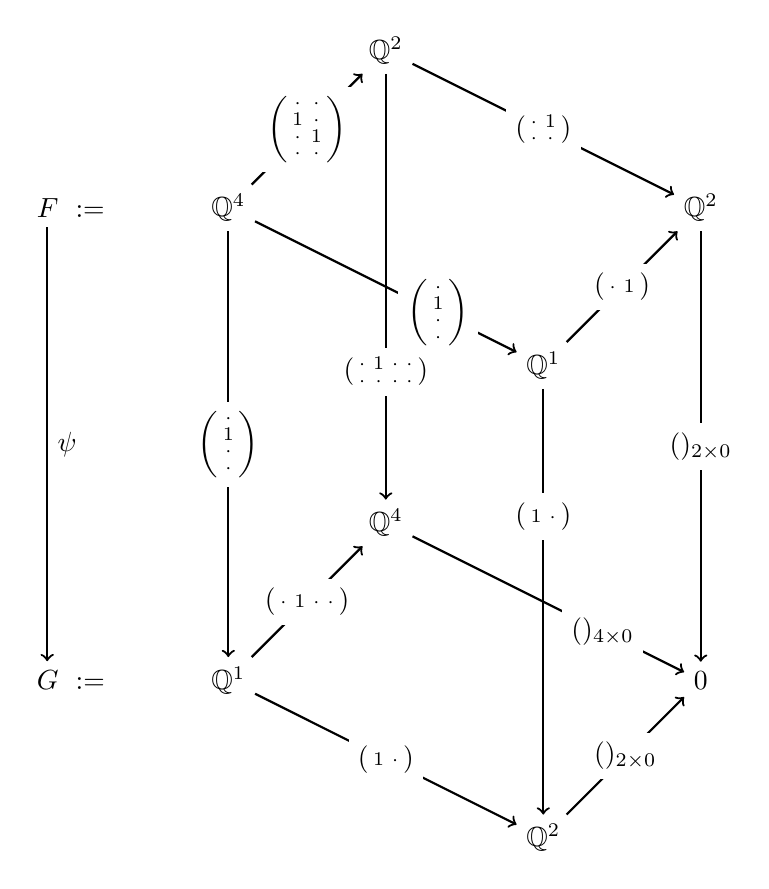
\begin{tikzpicture}[scale=1,transform shape,mylabel/.style={thick, draw=black, align=center,
            minimum width=0.5cm, minimum height=0.5cm,fill=red}]
            \coordinate (r) at (2,0);
            \coordinate (u) at (0,2);
            
            \node (F) at ($-2*(r)-1*(u)$) {$F~:=$};
            \node (2) at ($0*(r)+0*(u)$) {${\mathbb{Q}}^{2}$};
            \node (1) at ($-1*(r)-1*(u)$) {${\mathbb{Q}}^{4}$};
            \node (3) at ($1*(r)-2*(u)$) {${\mathbb{Q}}^{1}$};
            \node (4) at ($2*(r)-1*(u)$) {${\mathbb{Q}}^{2}$};
            
            \node (G) at ($-2*(r)-4*(u)$) {$G~:=$};
            \node (d2) at ($0*(r)-3*(u)$) {${\mathbb{Q}}^{4}$};
            \node (d1) at ($-1*(r)-4*(u)$) {${\mathbb{Q}}^{1}$};
            \node (d3) at ($1*(r)-5*(u)$) {${\mathbb{Q}}^{2}$};
            \node (d4) at ($2*(r)-4*(u)$) {${0}$};
            
            \path[->,thick] (F) edge[transform canvas={xshift=-0.3cm}] node[right]{$\psi$} (G);
           
            \path[->,thick] (2) edge node[fill=white, anchor=center, pos=0.7]{$\left( \begin{smallmatrix}
 \cdot & 1 & \cdot & \cdot \\ 
 \cdot & \cdot & \cdot & \cdot  
\end{smallmatrix} \right)$} (d2);

            \path[->,thick] (1) edge node[fill=white, anchor=center, pos=0.5]{$\left( \begin{smallmatrix}
 \cdot & \cdot \\ 
 1 & \cdot \\ 
 \cdot & 1 \\ 
 \cdot & \cdot 
\end{smallmatrix} \right)$} (2);

            \path[->,thick] (1) edge node[fill=white, anchor=center, pos=0.7]{$\left( \begin{smallmatrix}
 \cdot \\ 
 1 \\ 
 \cdot \\ 
 \cdot 
\end{smallmatrix} \right)$} (3);
            
            \path[->,thick] (2) edge node[fill=white, anchor=center, pos=0.5]{$\left( \begin{smallmatrix}
 \cdot & 1 \\ 
 \cdot & \cdot 
\end{smallmatrix} \right)$} (4);
            
            \path[->,thick] (3) edge node[fill=white, anchor=center, pos=0.5]{$\left( \begin{smallmatrix}
 \cdot & 1 
\end{smallmatrix} \right)$} (4);
         
             
             \path[->,thick] (d1) edge node[fill=white, anchor=center, pos=0.5]{$\left( \begin{smallmatrix}
 \cdot & 1 & \cdot & \cdot
\end{smallmatrix} \right)$} (d2);

            \path[->,thick] (d1) edge node[fill=white, anchor=center, pos=0.5]{$\left( \begin{smallmatrix}
 1 & \cdot
\end{smallmatrix} \right)$} (d3);
            
            \path[->,thick] (d2) edge node[fill=white, anchor=center, pos=0.7]{$()_{4 \times 0}$} (d4);
            
            \path[->,thick] (d3) edge node[fill=white, anchor=center, pos=0.5]{$()_{2 \times 0}$} (d4);
         
            \path[->,thick] (1) edge node[fill=white, anchor=center, pos=0.5]{$\left( \begin{smallmatrix}
 \cdot \\ 
 1 \\ 
 \cdot \\ 
 \cdot  
\end{smallmatrix} \right)$} (d1);

            \path[->,thick] (3) edge node[fill=white, anchor=center, pos=0.3]{$\left( \begin{smallmatrix}
 1 & \cdot 
\end{smallmatrix} \right)$} (d3);
            
            \path[->,thick] (4) edge node[fill=white, anchor=center, pos=0.5]{$()_{2 \times 0}$} (d4);

        \end{tikzpicture}
\end{document}
